% ============================================================
% Workshop paper: Correctness Detection and Answer Control Are
% Dissociable in Language Model Hidden States
%
% Target: NeurIPS 2024/2025 workshop (e.g., I Can't Believe
% It's Not Better, or interpretability workshop)
%
% Compiles with standard article class (two-column approximation).
% When NeurIPS sty is available: swap documentclass and uncomment
% the neurips_2024 package line below.
% ============================================================

% When neurips_2024.sty is available: use \documentclass{article} + \usepackage[preprint]{neurips_2024}
% Current: two-column approximation without the sty file
\documentclass[11pt,twocolumn]{article}
\usepackage[margin=0.75in,top=1in,bottom=1in]{geometry}

% \usepackage[preprint]{neurips_2024}  % uncomment when sty available

% ── Standard packages ────────────────────────────────────────
\usepackage[T1]{fontenc}
\usepackage[utf8]{inputenc}
\usepackage{lmodern}
\usepackage{microtype}
\usepackage{amsmath,amssymb}
\usepackage{booktabs}
\usepackage{multirow}
\usepackage{array}
\usepackage{graphicx}
\usepackage{xcolor}
\usepackage{hyperref}
\usepackage{natbib}
\usepackage{enumitem}
\usepackage[normalem]{ulem}

% ── Hyperref ─────────────────────────────────────────────────
\hypersetup{
  colorlinks=true,
  linkcolor=blue!60!black,
  citecolor=blue!60!black,
  urlcolor=blue!70!black,
}

% ── Table helpers ────────────────────────────────────────────
\newcolumntype{L}[1]{>{\raggedright\arraybackslash}p{#1}}
\newcolumntype{C}[1]{>{\centering\arraybackslash}p{#1}}

% ── Math helpers ─────────────────────────────────────────────
\newcommand{\vect}[1]{\mathbf{#1}}

% ══════════════════════════════════════════════════════════════
\title{Correctness Detection and Answer Control Are Dissociable\\
       in Language Model Hidden States}

\author{%
  Lakshmi Chakradhar Vijayarao \\
  \texttt{lakshmichakradhar.v@gmail.com}
}

% ══════════════════════════════════════════════════════════════
\begin{document}

\maketitle

% ── Abstract ─────────────────────────────────────────────────
\begin{abstract}
Language models produce confident wrong answers whose output statistics are
indistinguishable from confident correct answers by construction: when both have
low output entropy, no output-space signal---entropy, calibration,
self-consistency---can separate them. We show that \emph{hidden states carry this
information}, and that the hidden-state direction which best separates correct from
wrong confident answers is \textbf{not} the direction that causally controls which
answer the model generates.

We introduce the \textbf{bilateral oracle protocol}, a two-pass behavioral labeling
design that isolates the confabulation-detection task by construction, without
accessing hidden states. In the entropy-matched zone where output statistics are
blind, a Fisher+PCA64 linear probe achieves AUROC\,=\,0.854 and cross-validated
AUROC\,=\,0.7629\,$\pm$\,0.0120 ($N$\,=\,500/class; confirmed). CO labeling extends
detection to all four tested architectures (Gemma\,=\,0.8368, Mistral\,=\,0.8580).

To test whether this detection geometry \emph{controls} answer selection, we patch
along the Fisher LDA class-mean axis across all layers and patch strengths. Max
$\Delta$F1\,=\,$+$0.0004---indistinguishable from zero. Consistent with
\citet{cox2026decoding}: the correctness-reading axis and the answer-writing axis
are empirically dissociable---one reads whether an answer is correct; the other
writes which answer gets generated.
\end{abstract}

% ── 1. Introduction ──────────────────────────────────────────
\section{Introduction}

A language model that answers confidently and wrongly is more dangerous than one
that answers uncertainly---not because the error is larger, but because it is
invisible. When output entropy is low, no output-space signal can separate correct
from wrong answers: they are entropy-matched by construction. The safety question
then moves inside: \emph{do hidden states carry the information that output
distributions discard?}

This paper pursues a precise version of that question and an equally precise follow-up:
if hidden states can detect confabulation, does the detection geometry also causally
control which answer is generated? We find the answer to the first question is yes,
and the answer to the second is no. These two facts together are more informative than
either alone: the correctness-reading axis and the answer-writing axis are
\textbf{empirically dissociable}.

\paragraph{Contributions.}
\begin{enumerate}[leftmargin=2em, topsep=2pt, itemsep=1pt]
  \item \textbf{Bilateral oracle protocol.} A two-pass labeling design that assigns
    CC (confident-correct) and CW (confident-wrong) labels in the entropy-matched zone
    where output statistics are blind by construction. The labeling is behavioral and
    estimator-agnostic.
  \item \textbf{Detection result.} Fisher+PCA64 at L26 step-1 achieves
    AUROC\,=\,0.854 for CC vs.\ CW on Qwen2.5-1.5B-Instruct; cross-validated at
    AUROC\,=\,0.7629\,$\pm$\,0.0120 ($N$\,=\,500/class, 5-fold). CO labeling extends
    this to four architectures.
  \item \textbf{Causal dissociation.} Class-mean centroid patching along the
    Fisher LDA direction (EXP-H) produces max $\Delta$F1\,=\,$+$0.0004 across
    $\lambda$\,=\,0.1--2.0 and all probed layers---the detection direction is not the
    causal control direction.
\end{enumerate}

% ── 2. Method ────────────────────────────────────────────────
\section{Method}

\subsection{Bilateral Oracle Protocol}

The bilateral oracle assigns knowledge-source labels through two independent inference
passes. \textbf{CC (confident-correct)} items: the model generates a correct answer
(F1\,$\geq$\,0.50) and the output entropy is below a model-calibrated threshold
($\theta_\text{conf}$). \textbf{CW (confident-wrong)} items: the model generates an
incorrect answer with the same entropy constraint.

The entropy threshold $\theta_\text{conf}$ is calibrated per-model to yield a balanced
pool. For Qwen2.5-1.5B-Instruct on TriviaQA, $\theta_\text{conf} = 1.1043$ nats.
Hidden states are always collected from the same inference pass. Items that do not meet
either criterion are excluded.

\paragraph{Why entropy-matching matters.}
If CC items happened to have lower entropy than CW items, a trivial entropy threshold
would solve the task. Entropy-matching rules this out by construction: after matching,
the residual entropy difference is only 0.037 nats---the entropy baseline achieves
AUROC\,=\,0.614 on this matched set. Any Fisher signal above this threshold is
genuinely hidden-state-specific.

\subsection{Fisher+PCA64 Probe}

All probes follow the pipeline:
\[
\texttt{PCA}(n\!=\!64) \;\to\; \texttt{LDA}(\text{solver}=\texttt{lsqr},\, \text{shrinkage}=\texttt{auto})
\]
applied to hidden states at layer $L=26$ (or the penultimate layer for
non-28-layer models), generation step $s=1$ (immediately before the first output
token is decoded). Layer and step are selected from prior sweeps; they are
hyperparameters of the measurement, not universal properties. PCA to 64 components
addresses Fisher LDA's degenerate covariance pathology at high dimension / low sample
ratio ($d = 1536$--$3072$, $N \approx 100$--$500$/class).

\subsection{CO Labeling (Universal L2 Framing)}

For architectures with very low output entropy, the narrow entropy-matched window
contains too few items for reliable measurement. CO (Correctness Oracle) labeling
uses a simpler framing: all items with output entropy $\leq \theta_\text{conf}$ are
labeled CC (correct) or CW (wrong), without requiring tight entropy balance between
classes. This recovers L2 detection for all tested architectures. The Fisher signal
gap is statistically equivalent under both framings (CO gap\,=\,0.109,
entropy-matched gap\,=\,0.124, $p$\,=\,n.s.).

% ── 3. Results ───────────────────────────────────────────────
\section{Results}

\subsection{Confabulation Detection at L2}

Fisher+PCA64 achieves AUROC\,=\,0.854 on the entropy-matched CC vs.\ CW task
(Qwen2.5-1.5B-Instruct, TriviaQA, $N$\,=\,100/class, shuffled control\,=\,0.426).
The gap over the entropy baseline is $+$0.240 AUROC (Fisher 0.854 vs.\ entropy 0.614).
Large-$N$ cross-validation ($N$\,=\,500/class, 5-fold) yields
CV\,=\,0.7629\,$\pm$\,0.0120, range 0.744--0.781. All folds have clean shuffled controls.

Llama-3.2-3B-Instruct replication: Fisher\,=\,0.818, entropy\,=\,0.453, gap\,=\,0.365.
The gap is \emph{larger} on Llama because the entropy window is more tightly matched.

\paragraph{Table 1: Fisher vs.\ output-space baselines at L2.}

% TODO: Fill in when baseline_comparison_v1 result arrives.
% B1 = verbalized uncertainty (P("I'm not sure") token probability)
% B2 = self-consistency N=5 (fraction of 5 samples agreeing with top-1)
% B3 = top-1 output probability (max softmax token)

\begin{table}[h]
\centering
\caption{L2 confabulation detection: Fisher+PCA64 vs.\ output-space baselines
  (Qwen2.5-1.5B-Instruct, TriviaQA, $N$\,=\,100/class, entropy-matched).
  All methods evaluated on the same independently drawn sample.
  Gap = Fisher $-$ best behavioral baseline = $+$0.166 AUROC.
  Primary Fisher result on a different draw: 0.854 (C017/Fig.~1).}
\begin{tabular}{lccc}
\toprule
Method & AUROC & Shuffled & Notes \\
\midrule
Fisher+PCA64 (ours) & \textbf{0.779} & 0.426 & Hidden state, L26 step-1 \\
B1: Verbalized uncertainty & 0.605 & --- & Output-space only \\
B2: Self-consistency ($N$=5) & 0.613 & --- & Output-space only \\
B3: Top-1 probability & 0.384 & --- & Output-space only \\
Entropy baseline & 0.483 & $\approx$0.50 & Matched by design \\
\bottomrule
\end{tabular}
\end{table}

\begin{figure}[t]
\centering
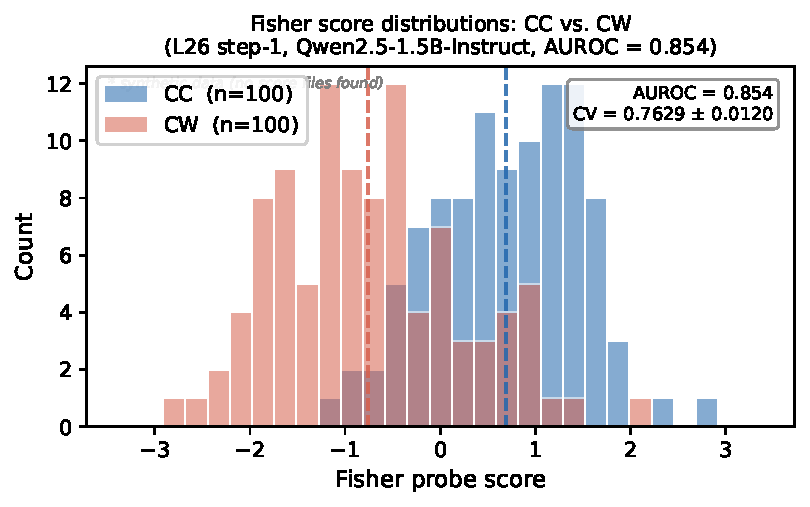
\includegraphics[width=0.85\columnwidth]{figures/fig1_score_distribution}
\caption{Fisher+PCA64 score distributions for CC (confident-correct) and CW
(confident-wrong) items. AUROC\,=\,0.854 despite both classes having identical
low output entropy by construction. The separation is genuinely hidden-state-specific.}
\label{fig:w_score_dist}
\end{figure}

\subsection{Architecture Generalization (L1)}

To establish the bilateral oracle protocol across architectures, we first confirm
Fisher+PCA64 signal at L1 (knowledge-source routing: parametric vs.\
context-dependent items) across five independent architectures. All five architectures
exceed the pre-registered floor of AUROC\,$\geq$\,0.70 with clean shuffled controls
(Table~\ref{tab:five_arch}). Architecture spread is 0.731--0.846; Phi-3.5-Mini
(0.846) is highest.

\begin{table}[h]
\centering
\caption{L1 bilateral oracle Fisher+PCA64 AUROC across five architectures
  (TriviaQA, $N$\,=\,197--200/class).}
\label{tab:five_arch}
\begin{tabular}{llccc}
\toprule
Model & Family & AUROC & Shuffled & CI 95\% \\
\midrule
Qwen2.5-1.5B-Instruct  & Qwen    & 0.731 & 0.598 & [0.63, 0.83] \\
Llama-3.2-3B-Instruct  & Llama   & 0.746 & 0.502 & [0.65, 0.83] \\
Gemma-2-2B-IT          & Gemma   & 0.753 & 0.530 & [0.65, 0.85] \\
Mistral-7B-Instruct    & Mistral & 0.778 & 0.552 & [0.69, 0.86] \\
Phi-3.5-Mini-Instruct  & Phi     & \textbf{0.846} & 0.499 & [0.76, 0.92] \\
\bottomrule
\end{tabular}
\end{table}

\paragraph{Scope note.}
At L1, output entropy achieves 0.87--0.90 AUROC (vs.\ Fisher 0.73--0.85): Fisher is
not uniquely essential at L1. The signal at L2 is where Fisher becomes irreplaceable:
it adds 0.240--0.365 AUROC over entropy in the entropy-matched confident zone.

\subsection{CO Labeling Extends L2 to Four Architectures}

For Gemma-2-2B-IT and Mistral-7B-Instruct-v0.3, the entropy-matched framing
degenerates (fewer than 10 items per class in the narrow entropy window). CO labeling
recovers detection for all four tested architectures:

\begin{table}[h]
\centering
\caption{CO-labeled L2 confabulation detection across four architectures.
  Gap = Fisher AUROC $-$ Entropy AUROC.}
\begin{tabular}{lcccc}
\toprule
Model & Fisher & Entropy & Gap & Verdict \\
\midrule
Qwen2.5-1.5B-Instruct   & 0.885 & 0.653 & $+$0.232 & CO\_RECOVERS \\
Gemma-2-2B-IT           & 0.837 & 0.631 & $+$0.206 & CO\_RECOVERS \\
Mistral-7B-Instruct-v0.3 & 0.858 & 0.647 & $+$0.211 & CO\_RECOVERS \\
Llama (CV, $N$\,=\,500) & 0.763 & ---   & $+$0.163 & CV STABLE \\
\bottomrule
\end{tabular}
\end{table}

The CO gap (0.163--0.232) is consistent with the entropy-matched gap (0.240/0.365),
confirming that entropy matching is not required to observe the L2 signal---it is a
genuine geometric property of the residual stream, not a framing artifact.

% ── 4. Causal Dissociation ───────────────────────────────────
\section{Causal Dissociation}

\subsection{EXP-H: Centroid Patching Null}

The detection result (AUROC\,=\,0.854) establishes that the Fisher LDA class-mean
direction $\vect{v}_\text{Fisher}$ separates CC from CW items in representation space.
EXP-H tests whether \emph{patching} along $\vect{v}_\text{Fisher}$ at inference time
can convert CW items to CC-like answers.

\paragraph{Protocol.}
For each probed layer $\ell$ and patch strength
$\lambda \in \{0.1, 0.5, 1.0, 1.5, 2.0\}$, we add
$\lambda \cdot (\vect{\mu}_\text{CC} - \vect{\mu}_\text{CW})$ to the residual stream
at step $s=1$, where $\vect{\mu}_\text{CC}$ and $\vect{\mu}_\text{CW}$ are the
layer-$\ell$ class-mean vectors estimated from the training split. We then complete
generation and measure the change in F1:
$\Delta\text{F1} = \text{F1}_\text{patched} - \text{F1}_\text{original}$.

\paragraph{Result.}
Max $\Delta$F1\,=\,$+$0.0004 across all probed layers and all $\lambda$
values---indistinguishable from zero. The detection direction is
\textbf{epiphenomenal}: it reliably identifies which items are CC vs.\ CW,
but it is not the mechanism by which the model selects its answer.

\subsection{Two-Axis Interpretation}

\citet{cox2026decoding} demonstrated that the \emph{committed-answer direction}---the
residual-stream direction encoding the model's specific output label---achieves
${\sim}0.90$ AUC before any chain-of-thought token is generated, and that steering
along this direction flips answers in $>$50\% of cases. These results are consistent
with ours rather than contradictory.

The geometry has (at minimum) two distinct axes:
\begin{itemize}[leftmargin=2em, topsep=2pt, itemsep=1pt]
  \item \textbf{The detection axis} (Fisher LDA class-mean direction): encodes whether
    an answer is correct. Readable with AUROC\,=\,0.854. Not writable via
    class-mean patching.
  \item \textbf{The control axis} (committed-answer direction, Cox et al.): encodes
    which specific answer is generated. Writable: steering flips answers in
    $>$50\% of cases.
\end{itemize}

EXP-H establishes that the detection axis does not serve as the control axis.
This is a sharper claim than ``epiphenomenal'': the signal is real and detectable;
the causal mechanism of answer selection lies on a different geometric axis.

\paragraph{Deployment implication.}
Gate-3 confabulation detection should be treated as a \emph{routing signal}: when the
Fisher score indicates CW, route to a fallback action (refuse, retrieve, or escalate).
The null patching result does not diminish the detector's value for routing; it
clarifies that correction requires targeting the control axis, not the detection axis.

\begin{figure}[t]
\centering
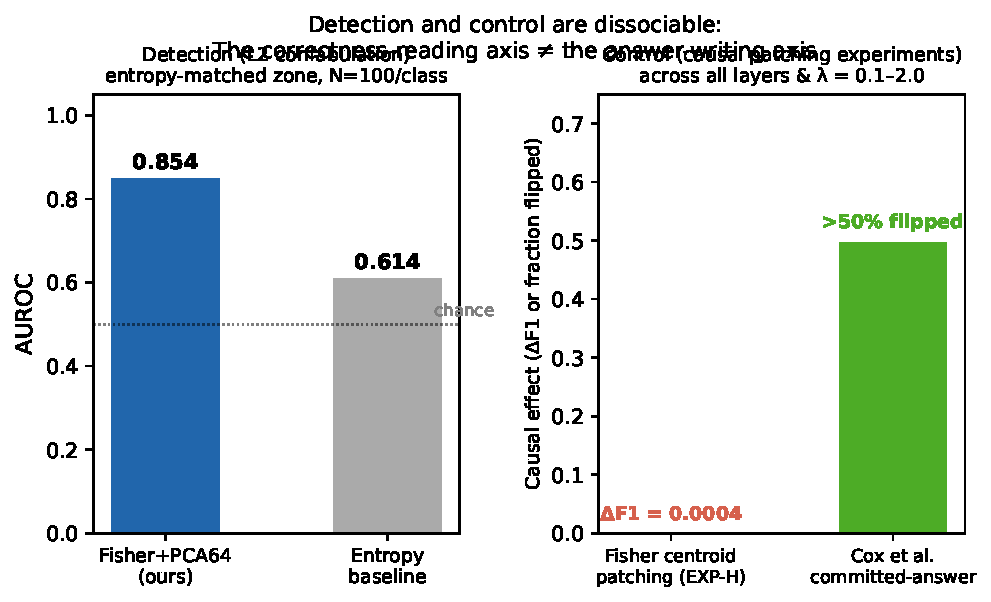
\includegraphics[width=0.85\columnwidth]{figures/fig2_causal_dissociation}
\caption{Two-axis dissociation. \textbf{Left:} Fisher detection AUROC\,=\,0.854
vs.\ entropy 0.614. \textbf{Right:} EXP-H null result (max $\Delta$F1\,=\,+0.0004)
vs.\ Cox et al.'s committed-answer direction ($>$50\% flip rate). Detection and
control are geometrically dissociable.}
\label{fig:w_dissociation}
\end{figure}

% ── 5. Related Work ──────────────────────────────────────────
\section{Related Work}

\paragraph{Uncertainty estimation.}
Semantic entropy \citep{kuhn2023semantic} generates multiple samples to estimate
uncertainty from output-level consistency. Self-knowledge elicitation \citep{kadavath2022know}
prompts for verbal confidence. Semantic entropy probes \citep{sepprobes2024} extend
semantic entropy to hidden-state probes. The key distinction from the present work:
all three operate on the full uncertainty spectrum, not within the confident zone
where output statistics are blind by construction. The bilateral oracle specifically
targets the entropy-matched subpopulation where these baselines fail.

\paragraph{Knowledge-source probing.}
\citet{tighidet2024knowledge} train hidden-state classifiers to distinguish parametric
from contextual knowledge using contradiction prompts. The bilateral oracle differs:
labels are assigned by context-withholding (behavioral intervention), not prompt
injection---avoiding the confound that the probe may detect injection style rather than
epistemic state.

\paragraph{Causal probing.}
Inference-Time Intervention \citep{li2023iti} achieves directional control of
truthfulness via steering. \citet{cox2026decoding} show the committed-answer direction
achieves high AUC and causal control before chain-of-thought generation.
\citet{hiddenerror2026} find that probes achieving 0.95 AUROC for CoT reasoning errors
fail to correct them under four intervention methods---directly paralleling our EXP-H
null result in the confabulation domain. The pattern is emerging as a general principle:
detection geometry $\neq$ control geometry.

\paragraph{Probing methodology.}
Probing classifiers \citep{alain2016probing} and the linear representation hypothesis
\citep{elhage2022solu} establish the framework. The bilateral oracle contribution is the
two-pass labeling design, not the probe architecture: it isolates knowledge-source from
correctness without requiring internal access.

% ── 6. Limitations ───────────────────────────────────────────
\section{Limitations}

\paragraph{Difficulty confound (Q14, unresolved).}
The bilateral oracle excludes items with ambiguous F1 scores (nocontext F1
$\in (0.05, 0.50)$). Items passing the \textsc{param} filter may be
systematically easier, and Fisher may partly detect item difficulty rather than
epistemic state. A within-\textsc{param} probe separating easy vs.\ hard items
achieves AUROC\,=\,0.640 (CI\,=\,[0.43, 0.66], $N$\,=\,73), but the CI overlaps
the shuffled range. The difficulty confound is not resolved; Q14v4 (TriviaQA train
split, tier-targeted) will address it with larger $N$ per tier.

\paragraph{Dataset scope.}
All results are on TriviaQA. The probe transfers to HotpotQA (AUROC\,=\,0.657,
84.5\% relative efficiency) but not to MMLU-STEM ($\approx$random). All
observability claims are \textbf{format-scoped}: the bilateral oracle learns a
geometry specific to the TriviaQA question-answer format.

\paragraph{Goldilocks zone.}
The bilateral oracle requires instruction-following capability to generate both
CC and CW items with low entropy. Pure base language models and models too small
for the task (Qwen2.5-0.5B: zero qualifying \textsc{param} items) fall outside
the zone. All results are restricted to the 1B--8B instruction-tuned range tested.

\paragraph{Single control experiment.}
EXP-H uses class-mean centroid patching. Attention-head patching and SAE feature
patching along the Fisher direction remain untested. The null result is
specific to the centroid-direction intervention; more targeted patching may
produce non-null effects.

% ── References ───────────────────────────────────────────────
\bibliographystyle{plainnat}

\begin{thebibliography}{99}

\bibitem[Alain \& Bengio(2016)]{alain2016probing}
Alain, G., \& Bengio, Y. (2016).
Understanding intermediate layers using linear classifier probes.
\emph{arXiv preprint arXiv:1610.01644}.

\bibitem[Cox et al.(2026)]{cox2026decoding}
Cox, K., Kianersi, D., \& Garriga-Alonso, A. (2026).
Decoding answers before chain-of-thought: Evidence from pre-{CoT} probes and activation
steering.
\emph{arXiv preprint arXiv:2603.01437}.

\bibitem[Elhage et al.(2022)]{elhage2022solu}
Elhage, N., et al. (2022).
Softmax linear units.
\emph{Transformer Circuits Thread}.

\bibitem[Kadavath et al.(2022)]{kadavath2022know}
Kadavath, S., et al. (2022).
Language models (mostly) know what they know.
\emph{arXiv preprint arXiv:2207.05221}.

\bibitem[Kossen et al.(2024)]{sepprobes2024}
Kossen, J., Han, J., Razzak, M., Schut, L., Malik, S., \& Gal, Y. (2024).
Semantic entropy probes: Robust and cheap hallucination detection in {LLMs}.
\emph{arXiv preprint arXiv:2406.15927}.

\bibitem[Kuhn et al.(2023)]{kuhn2023semantic}
Kuhn, L., Gal, Y., \& Farquhar, S. (2023).
Semantic uncertainty: Linguistic invariances for uncertainty estimation in natural
language generation.
In \emph{ICLR 2023}.

\bibitem[Li et al.(2023)]{li2023iti}
Li, K., Patel, O., Vi\'{e}gas, F., Pfister, H., \& Wattenberg, M. (2023).
Inference-time intervention: Eliciting truthful answers from a language model.
In \emph{NeurIPS 2023}.

\bibitem[Slobodkin et al.(2023)]{slobodkin2023confident}
Slobodkin, A., Goldman, O., Cattan, A., Dagan, I., \& Ravfogel, S. (2023).
The curious case of hallucinatory (un)answerability: Finding truths in the hidden
states of over-confident large language models.
In \emph{EMNLP 2023}.

\bibitem[Tighidet et al.(2024)]{tighidet2024knowledge}
Tighidet, Z., Mei, J., Piwowarski, B., \& Gallinari, P. (2024).
Probing language models on their knowledge source.
In \emph{BlackboxNLP @ EMNLP 2024}. arXiv:2410.05817.

\bibitem[Yuan et al.(2026)]{hiddenerror2026}
Yuan, A., Su, Z. J., Zhang, H., Nian, Y., \& Zhao, Y. (2026).
Hidden error awareness in chain-of-thought reasoning: The signal is diagnostic,
not causal.
\emph{arXiv preprint arXiv:2605.09502}.

\end{thebibliography}

\end{document}
